\section{Objetivos}
\label{sec:objetivos}
Un actuador es un dispositivo capaz de transformar energía (eléctrica para nuestro caso de interés) en la activación de un proceso con la finalidad de generar un efecto sobre un proceso automatizado. Al mismo tiempo, existe un controlador que se encarga de enviar ordenes al actuador con las cuales se activa un elemento final de control. Un ejemplo de actuador utilizado frecuentemente son los actuadores piezoeléctricos, los cuales producen una deformación mecánica sobre el material piezoeléctrico a partir de la aplicación de un campo eléctrico externo y viceversa. Estos tipos de actuadores pueden funcionar como por ejemplo, microposicionadores.

En este proyecto se busca diseñar un actuador que se utilizará en un esquema interferométrico, más precisamente en un interferómetro de Michelson. Este tipo de esquema se describe en la figura \ref{fig:interferometro}.

\begin{figure}[H]
  \centering
  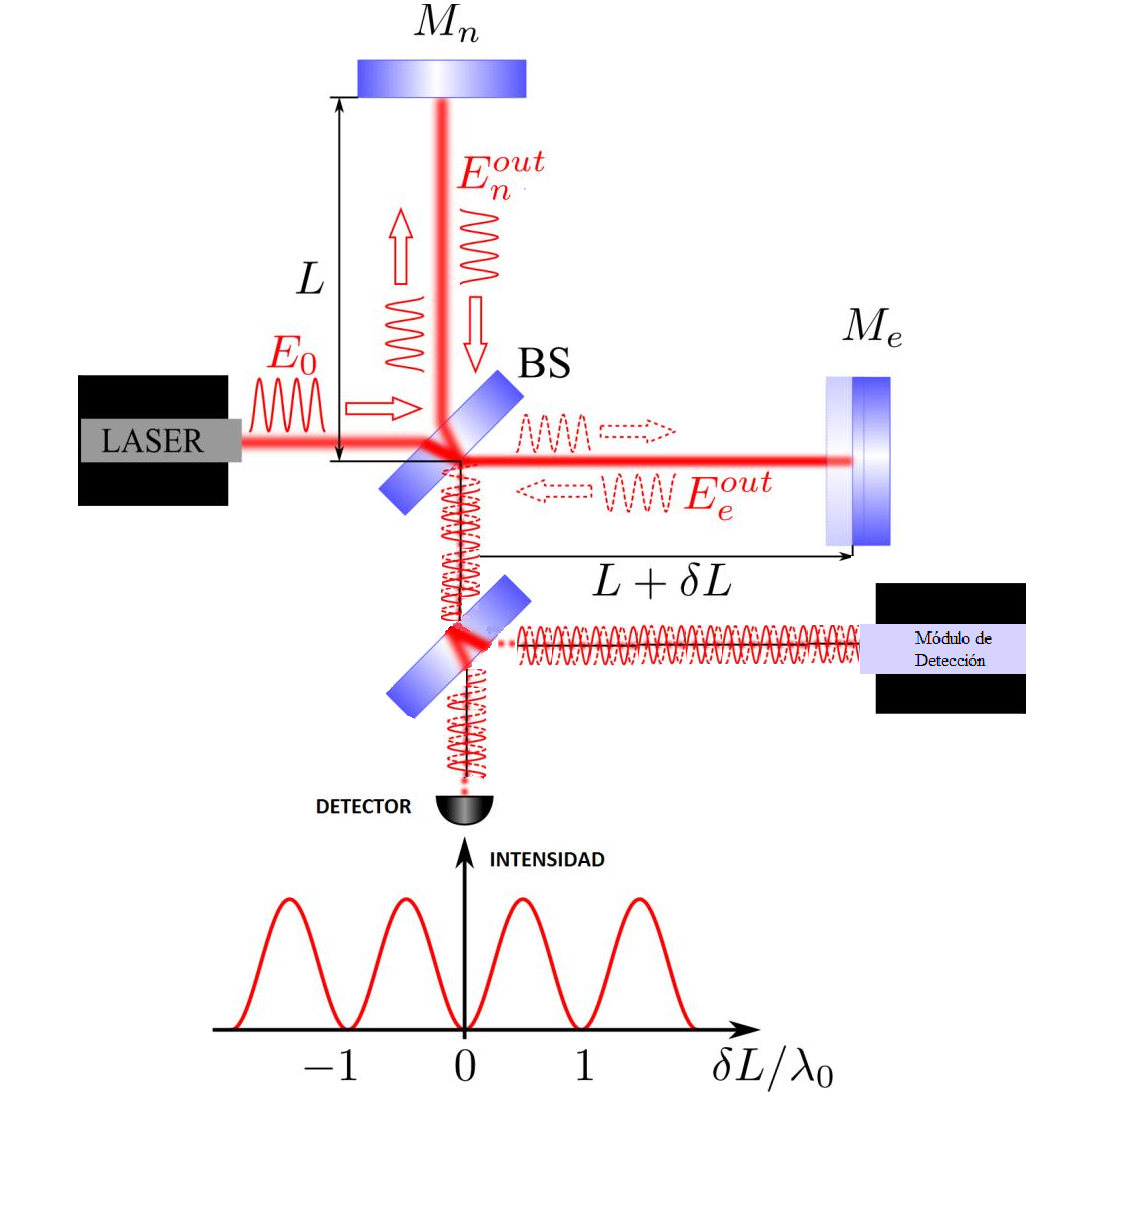
\includegraphics[width=0.6\textwidth]{images/interfer_metro+modulo_deteccion.png}
  \caption{Interferómetro de Michelson}
  \label{fig:interferometro}
\end{figure}

%% Modificar la figura y agregar el modulo de deteccion que va a l micro (y tambien aclalarlo en el texto)%%

Mediante un divisor de haz ($BS$), se superponen dos campos proveniente de un fuente monocromática y coherente ($laser$). El campo que se desvía hacia la rama superior se refleja mediante un espejo fijo ($M_n$) mientras que el campo que se desvía hacia la derecha se refleja en un espejo móvil ($M_e$). De esta manera, los campos reflejados se dirigen hacia la rama inferior, donde se superponen en un fotodetector por medio del cual se puede registrar la intensidad de estos dos campos superpuestos. El modelo de esta intensidad es el siguiente:

\begin{equation}
I(t) = A + B \enspace cos\left[\frac{4 \pi}{\lambda_0} (L_1 - (L_2 + \delta L(t)) \ )\right]
\label{eq:prin}
\end{equation}

donde $L_1$, $L_2$ y $\delta L$ son las que se muestran en la figura \ref{fig:interferometro}, y $\lambda_0$ es la longitud de onda del haz incidente.

De esta manera, con la ayuda del fotodetector se puede medir la intensidad producida por la diferencia de camino óptico ($\delta L$).
Si las ramas del interferómetro tienen la misma distancia (es decir, $L_1 = L_2 = L$), la intensidad registrada sólo depende del movimiento del espejo móvil $\delta L$.

Por lo tanto: Existe una variación de la intensidad detectada producto del desplazamiento del espejo móvil. Si conocemos $A$, $B$ y la longitud de onda de la fuente es posible recuperar la información del desplazamiento producido por $M_e$ midiendo la intensidad en el detector. Claramente este proceso también puede aplicarse de manera inversa, esto es: si podemos controlar con una resolución elevada la posición del espejo podemos determinar la longitud de onda de la fuente lumínica y los parámetros $A$ y $B$.